\documentclass[9pt]{beamer}

\usetheme[progressbar=frametitle]{metropolis}
\usepackage{appendixnumberbeamer}

\usepackage{booktabs}
\usepackage[scale=2]{ccicons}

\usepackage{pgfplots}
\usepgfplotslibrary{dateplot}
\usepackage{xcolor}
\usepackage{soul}

\usepackage{listings}

\lstset{
    language=Python,
    basicstyle=\ttfamily\small,
    keywordstyle=\color{blue},
    commentstyle=\color{gray},
    stringstyle=\color{red},
    showstringspaces=false,
    breaklines=true
}

\usepackage{xspace}
\newcommand{\themename}{\textbf{\textsc{metropolis}}\xspace}

\title{Monte Carlo Methods }
\subtitle{with Applications in Finance}
\date{\today}

\author{Chin Zhe Ning\inst{1}}
\institute{
\inst{1} National University of Singapore \\ Prof. Ren Weiqing
}
% \titlegraphic{\hfill\includegraphics[height=1.5cm]{logo.pdf}}

\begin{document}

\maketitle

\begin{frame}{Table of contents}
  \setbeamertemplate{section in toc}[sections numbered]
  \tableofcontents%[hideallsubsections]
\end{frame}

\section[Introduction]{Introduction}
\begin{frame}{Derivatives}
\begin{itemize}
    \item A derivative is a security whose value depends on an underlying asset, a group of assets, or a benchmark.
    \item Analytical solutions exist for simple derivatives (e.g., Black-Scholes formula for European call options).
    \item Complex derivatives (path-dependent or multi-asset) are often impossible to solve analytically.
\end{itemize}
\end{frame}

\begin{frame}{Monte Carlo Methods in Finance}
\begin{itemize}
    \item Monte Carlo methods estimate expected payoffs by simulating many random scenarios.
    \item Well-suited for path-dependent and multi-asset derivatives.
    \item Advantages: robust, flexible, handles high-dimensional problems.
    \item Limitations: slow convergence, high computational cost for precise estimates.
\end{itemize}
\end{frame}

\section[Option Pricing]{Option Pricing}

\begin{frame}{Risk-Neutral Valuation}
Suppose the payoff of a derivative is a function $h(X)$ of a random variable $X$ related to the underlying asset. 

By the principle of no-arbitrage\cite{merton1973rational, black1973pricing}, the derivative's price is the expected discounted payoff under a risk-neutral measure:
\[
v = \mathbb{E}[e^{-r T} h(X)],
\]
where
\begin{itemize}
    \item $r$ is the \textit{risk-free interest rate}, 
    \item $T$ is the time to maturity.
\end{itemize}

Under this measure, all assets are expected to grow at the risk-free rate, reducing pricing to computing expected discounted payoffs.
\end{frame}

\begin{frame}{Underlying Asset Model}
The underlying asset price is commonly modeled as a geometric Brownian motion:
\[
S_t = S_0 \exp \Big( (r - \tfrac{1}{2} \sigma^2) t + \sigma W_t \Big), \quad W_t \sim N(0,t),
\]
where
\begin{itemize}
    \item $S_0$ is the initial price,
    \item $\sigma$ is the volatility (constant), and
    \item $W_t$ is a standard Brownian motion.
\end{itemize}

This model will be assumed throughout this report.
\end{frame}

\begin{frame}{Examples of Derivative Payoffs}
\begin{enumerate}
    \item \textbf{European Call Option:} Strike $K$, underlying $S_T$, discounted payoff:
    \[
    h(S_T) = e^{-r T} (S_T - K)^+, \quad v = \mathbb{E}[h(S_T)].
    \]
    Closed-form solution via Black-Scholes formula\cite{black1973pricing}:
    \[
    v = S_0 \Phi(\sigma\sqrt{T} - \theta) - K e^{-r T} \Phi(-\theta),
    \]
    with $$\theta = \frac{1}{\sigma \sqrt{T}} \ln \frac{K}{S_0} + (\frac{\sigma}{2} - \frac{r}{\sigma}) \sqrt{T}.$$
    
    \item \textbf{Asian Call Option:} Discretely monitored average price option, payoff:
    \[
    h(S_{t_1},\dots,S_{t_m}) = e^{-r T} \Big(\frac{1}{m} \sum_{i=1}^{m} S_{t_i} - K\Big)^+.
    \]
    Closed-form solutions exist only in special cases (e.g. geometric average price option); and no analytical solution is available \cite{kemna1990pricing}.
\end{enumerate}

\smallskip
Monte Carlo methods can be used to estimate $v$ by approximating the expected payoff through random sampling.
\end{frame}


\section[Plain Monte Carlo Method]{Plain Monte Carlo Method}

\begin{frame}{Monte Carlo Estimator}
\small
\textbf{Problem:} Estimate the quantity
\(v = \mathbb{E}[X],\)
where \(X = h(Z)\) is a function of a r.v. \(Z\).

\textbf{Plain Monte Carlo estimator:}
\begin{itemize}
    \item Generate \(N\) i.i.d. samples \(Z_i \sim f_Z\), $i = 1, ..., N$.
    \item Compute the sample mean
    \[
    \hat{v} = \frac{1}{N} \sum_{i=1}^{N} h(Z_i).
    \]
    \item \(\hat{v}\) is unbiased:
    \[
    \mathbb{E}[\hat{v}] = v, \quad \mathrm{Var}(\hat{v}) = \frac{\mathrm{Var}(X)}{N}.
    \]
\end{itemize}

As \(N\) increases, \(\hat{v}\) converges to the true mean \(v\).
\end{frame}

\begin{frame}{Examples: European Call Option}
\small
\textbf{European Call Option:} Strike \(K = 60\), maturity \(T = 1\) year. Discounted payoff:
\[
h(S_T) = e^{-rT} (S_T - K)^+.
\]

\textbf{Parameters:} \(S_0 = 50, r = 0.05, \sigma = 0.2\) drive the Geometric Brownian Motion.

\begin{table}[ht]
\centering
\begin{tabular}{c c c c c c}
\toprule
$N$ & $10^2$ & $10^3$ & $10^4$ & $10^5$ & $10^6$ \\
\midrule
Estimate & 1.8824 & 1.6428 & 1.6586 & 1.6119 & 1.6181 \\
S.E. & 0.6072 & 0.1388 & 0.0447 & 0.0135 & 0.0043 \\
R.E. & 32.25\% & 8.45\% & 2.69\% & 0.84\% & 0.27\% \\
\bottomrule
\end{tabular}
\caption{European Call Option: Monte Carlo estimates for different sample sizes $N$}
\end{table}

\textbf{Note.} Convergence to \(v = 1.6237\)  as \(N\) increases.
\end{frame}

\begin{frame}{Examples: Asian Call Option}
\small
\textbf{Asian Call Option:} Discretely monitored with \(m = 100\) time points, strike \(K = 60\), maturity \(T=1\), discounted payoff:
\[
h(S_{t_1},\dots,S_{t_m}) = e^{-rT} \left( \frac{1}{m} \sum_{i=1}^{m} S_{t_i} - K \right)^+.
\]

\textbf{Parameters:} \(S_0=50, r=0.05, \sigma=0.2\).

\begin{table}[ht]
\centering
\begin{tabular}{c c c c c c}
\toprule
$N$ & $10^2$ & $10^3$ & $10^4$ & $10^5$ & $10^6$ \\
\midrule
Estimate & 0.2823 & 0.2534 & 0.2650 & 0.2715 & 0.2700 \\
S.E. & 0.1224 & 0.0357 & 0.0122 & 0.0040 & 0.0013 \\
R.E. & 43.36\% & 14.09\% & 4.60\% & 1.47\% & 0.47\% \\
\bottomrule
\end{tabular}
\caption{ Asian Call Option: Monte Carlo estimates for various \(N\)}
\end{table}

\end{frame}

\begin{frame}{Limitations of Plain Monte Carlo}
\small
\metroset{block=fill}
\begin{alertblock}{Rate of Convergence}
        By the \textit{Central Limit Theorem}, for large \(N\):
        \[
        \sqrt{N} (\hat{v} - v) \xrightarrow{d} \mathcal{N}(0, \sigma^2)
        \]
        where \(\sigma^2 = \mathrm{Var}(X)\). So convergence is \textbf{slow}. \(\text{S.E.}(\hat{v}) = \mathcal{O}(N^{-1/2})\).
      \end{alertblock}
\begin{itemize}
    \item High variance \(\sigma^2\) increases with problem dimension or payoff complexity\footnote{Example: Deep out-of-the-money options lead to skewed payoff distributions and large relative errors.}.
    \item Large sample sizes needed for high precision, computationally expensive.
\end{itemize}
\end{frame}

\begin{frame}
\begin{center}
\begin{figure}
    \centering
    \includegraphics[width=0.75\linewidth]{assets/plain-monte-carlo-se-vs-sample-size.png}
    \caption{Plain Monte Carlo: Standard Error (S.E.) vs Sample Size $N$}
    \label{fig:placeholder}
\end{figure}
\end{center}
\end{frame}

\begin{frame}{Motivation for Variance Reduction}
\small
\begin{figure}
    \centering
    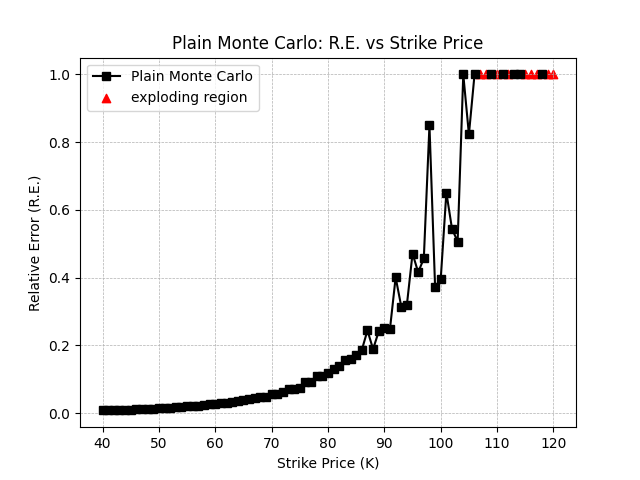
\includegraphics[width=0.75\linewidth]{assets/plain-monte-carlo-re-vs-strike-price.png}
    \caption{Plain Monte Carlo: R.E. versus Strike Price, $N=10{,}000$}
\end{figure}
\begin{itemize}
    \item Deep out-of-the-money option when $K \gg S_0$. Frequency of exercising low. Variance $\sigma^2$ high. Slow convergence.
\end{itemize}

\end{frame}

\begin{frame}
\small
\begin{itemize}
    \item Increasing \(N\) to reduce standard error is expensive: a 10x reduction in S.E. requires 100x more samples.
    \item \textbf{Variance reduction techniques} aim to lower the estimator variance \(\sigma^2\) without increasing \(N\).
    \item Popular methods: Antithetic sampling, Control variates, Stratified sampling, Importance sampling, \hl{Control functionals} (recent approach)
    \item Other advanced methods: quasi-Monte Carlo\footnote{Quasi–Monte Carlo replaces random samples with deterministic low-discrepancy sequences (e.g., Sobol’, Halton), reducing integration error without relying on randomness.}, multi-level Monte Carlo.
\end{itemize}
\end{frame}

\section[Variance Reduction Techniques]{Variance Reduction Techniques}

% \subsection{Antithetic Sampling}

% \begin{frame}{Antithetic Sampling: Idea}
% \small
% Generate i.i.d. pairs \((X_i, Y_i)\) such that:

% \begin{enumerate}[i.]
%     \item \(X_i\) and \(Y_i\) have the same distribution.
%     \item \(X_i\) and \(Y_i\) are \textbf{negatively correlated}.
% \end{enumerate}

% \[
% \hat{v}_{\text{AS}} = \frac{1}{N} \sum_{i=1}^{N} \frac{X_i + Y_i}{2}
% \]

% \begin{itemize}
%     \item If \(\beta = \text{Corr}(X, Y) < 0\), then
%     \[
%     \text{Var}[\hat{v}_{\text{AS}}] = \frac{(1+\beta)\text{Var}[X]}{2N} < \frac{\text{Var}[X]}{2N}.
%     \]
%     \item Stronger negative correlation → greater variance reduction.
% \end{itemize}

% \footnotesize{In practice, antithetic pairs are often generated as \(X_i = h(U_i)\), \(Y_i = h(1-U_i)\) with \(U_i \sim \text{Uniform}(0,1)\) and monotone \(h\).}
% \end{frame}

% \begin{frame}{European Call Option Example}
% \small
% \textbf{European Call Option:} 
% $$S_T = S_0 \exp((r- \frac{1}{2}\sigma^2)T + \sigma \sqrt{T} Z), \quad Z \sim N(0,1).$$  

% \begin{itemize}
%     \item Generate antithetic samples: \(X_i = h(S_T(Z_i))\), \(Y_i = h(S_T(-Z_i))\).
%     \item Compare plain MC vs antithetic sampling for \(N=10{,}000\) and \(S_0 = 40,50,60\).
% \end{itemize}

% \begin{table}[ht]
% \centering
% \begin{tabular}{c|cc|cc|cc}
% \toprule
% Strike Price & \multicolumn{2}{c|}{$S_0 = 40$} & \multicolumn{2}{c|}{$S_0 = 50$} & \multicolumn{2}{c}{$S_0 = 60$} \\
%  & Plain MC & AS & Plain MC & AS & Plain MC & AS \\
% \midrule
% Estimate & 12.3593 & 12.2832 & 5.2996 & 5.4026 & 1.6731 & 1.6009 \\
% S.E. & 0.0950 & 0.0233 & 0.0731 & 0.0385 & 0.0442 & 0.0285 \\
% R.E. & 0.77\% & 0.19\% & 1.38\% & 0.71\% & 2.64\% & 1.78\% \\
% \bottomrule
% \end{tabular}
% \caption{European Call Option: Estimates, standard errors (S.E.) and relative errors (R.E.) using Plain Monte Carlo (Plain MC) and Antithetic Sampling (AS) for different initial stock prices $S_0$.}
% \end{table}


% \end{frame}

% \begin{frame}{Straddle Option Example}
% \small
% \textbf{Straddle Option:} Combination of call and put with the same strike \(K\):  
% \[
% h(S_T) = (S_T - K)^+ + (K - S_T)^+
% \]

% \begin{itemize}
%     \item Antithetic pairs generated as in the European call example.
%     \item Parameters: \(K = 50, r=0.02, \sigma=0.2, T=1\), sample size \(N=10{,}000\).
% \end{itemize}

% \begin{table}[ht]
% \centering
% \small
% \begin{tabular}{c|cc|cc|cc}
% \toprule
% Strike Price & \multicolumn{2}{c|}{$S_0 = 40$} & \multicolumn{2}{c|}{$S_0 = 50$} & \multicolumn{2}{c}{$S_0 = 60$} \\
%  & Plain MC & AS & Plain MC & AS & Plain MC & AS \\
% \midrule
% Estimate & 10.3312 & 10.4426 & 7.9219 & 8.2118 & 12.8876 & 12.7170 \\
% S.E. & 0.0614 & 0.0347 & 0.0626 & 0.0897 & 0.1035 & 0.0702 \\
% R.E. & 0.59\% & 0.33\% & 0.79\% & 1.09\% & 0.80\% & 0.55\% \\
% \bottomrule
% \end{tabular}
% \caption{Straddle Option: Antithetic Sampling (AS) vs Plain Monte Carlo (Plain MC) estimates, standard error (S.E.), and relative error (R.E.) for different initial stock prices $S_0$.}
% \end{table}

% \end{frame}

% \begin{frame}{Straddle Option: Relative Error}
% \small
% \begin{itemize}
%     \item For \(S_0\) far from \(K\), antithetic sampling reduces variance.
%     \item For \(S_0\) near \(K\), correlation becomes positive, reducing effectiveness.
% \end{itemize}

% \begin{figure}
% \centering
% 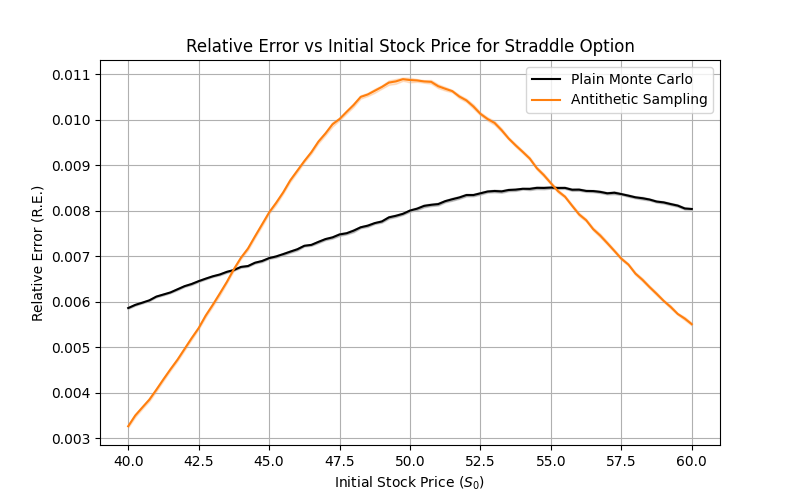
\includegraphics[width=0.75\textwidth]{assets/straddle-option-re-vs-initial-stock-price.png}
% \caption{Straddle Option: Relative error of antithetic sampling vs plain MC as $S_0$ varies from 40 to 60.}
% \end{figure}
% \end{frame}

% \begin{frame}{Limitations of Antithetic Sampling}
% \small
% \begin{itemize}
%     \item Works well when payoff \(h\) is monotonic (e.g., European call).
%     \item For non-monotonic payoffs (e.g., straddle option), correlation can be weak or positive. Variance increases.
% \end{itemize}

% \begin{figure}
% \centering
% 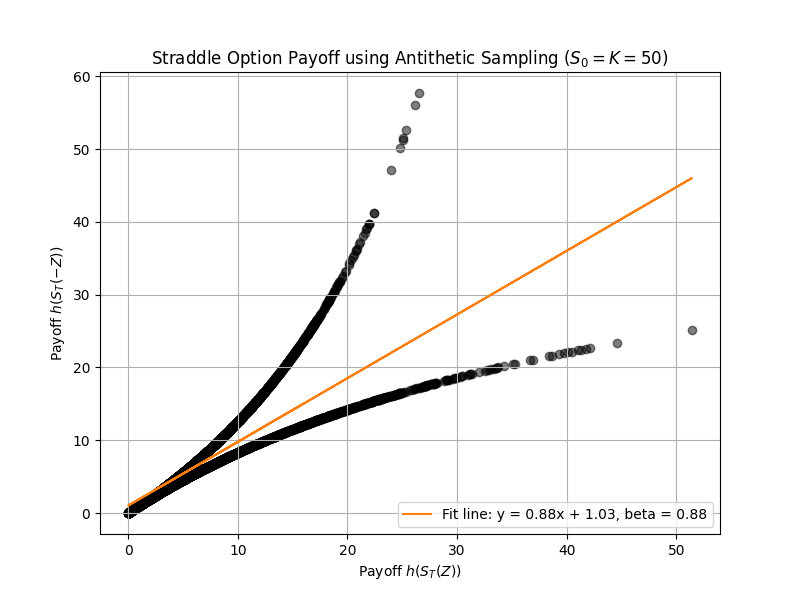
\includegraphics[width=0.7\textwidth]{assets/straddle-option-antithetic-scatter.png}
% \caption{Payoff function $h(S_T)$ vs $S_T$ for straddle option, $S_0 = K = 50$, showing positive correlation of antithetic pairs.}
% \end{figure}
% \end{frame}

\subsection{Control Variates}

\begin{frame}{Control Variates: Concept}
\small
Suppose a r.v. $Y$ exists such that:
\begin{enumerate}[i.]
    \item $X$ and $Y$ are correlated;
    \item generating $Y_i$ from $X_i$ is cheap;
    \item the expected value $\mathbb{E}[Y]$ is known exactly.
\end{enumerate}

\textbf{Control Variate (CV) Estimator:}
\[
\hat{v}_{\text{CV}} = \bar{X} - b (\bar{Y} - \mathbb{E}[Y]),
\]
where $\bar{X}$, $\bar{Y}$ are sample means, and $b$ is chosen to minimize variance\footnote{Typically, $b^*$ is computed from a smaller pilot sample.}:
\[
b^* = \frac{\text{Cov}[X,Y]}{\text{Var}[Y]}.
\]

Variance of the estimator:
\[
\text{Var}[\hat{v}_{\text{CV}}] = (1-\beta^2) \frac{\text{Var}[X]}{N},
\]
where $\beta$ is the correlation between $X$ and $Y$.
\end{frame}

% Asian Option example
\begin{frame}{Asian Option: Control Variates vs Plain MC}
\small
\textbf{Asian Call Option:} Discretely monitored with $m = 100$ time points $0 < t_1 < \cdots < t_m = T$, maturity $T = 1$, discounted payoff:
$$X = h(S_{t_1}, ..., S_{t_m}) = e^{-r T} \left( \bar{S} - K\right)^+, \quad \bar{S} = \frac{1}{m} \sum_{i = 1}^m S_{t_i}. $$

\textbf{Parameters:} $S_0 = 50$, $r = 0.05, \sigma = 0.2, T = 1$, and $N = 10{,}000$.

\textbf{Control Variate:} Average price call option with geometric mean. Discounted payoff:
$$ Y = e^{-rT } (\bar{S}_G - K)^+, \quad \bar{S}_G = \left( \prod_{i = 1}^m S_{t_i} \right)^{1/m.}. $$
The mean is known, see \textit{Example 2.5.} in \cite{textbook}:
$$\bar{\mu} = \log S_0 + (r - \frac{\sigma^2}{2})\frac{1}{m}\sum_{i = 1}^{m}  t_i,$$
$$\bar{\sigma}^2 = \frac{\sigma^2}{m^2} \sum_{i = 1}^{m} (2m - 2i + 1)t_i. $$
$$E[Y] = e^{-rT} [e^{\bar{\mu} + \frac{1}{2} \bar{\sigma}^2} \Phi(\bar{\sigma} - \theta) + K \Phi(-\theta)], \quad \theta = (\log K - \bar{\mu})/\bar{\sigma}$$

\end{frame}

\begin{frame}
\small
\begin{table}[ht]
\centering
\begin{tabular}{c|cc|cc|cc}
\toprule
Strike Price & \multicolumn{2}{c|}{$K = 60$} & \multicolumn{2}{c|}{$K = 70$} & \multicolumn{2}{c}{$K = 80$} \\
 & Plain MC & CV & Plain MC & CV & Plain MC & CV \\
\midrule
Estimate & 0.2887 & 0.2720 & 0.0159 & 0.0107 & 0.0000 & 0.0009 \\
S.E. & 0.0130 & 0.0009 & 0.0032 & 0.0005 & 0.0000 & 0.0001 \\
R.E. & 4.51\% & 0.33\% & 19.83\% & 4.26\% & nan\% & 13.39\% \\
Variance Reduction & \multicolumn{2}{c|}{99.53\%} & \multicolumn{2}{c|}{97.92\%} & \multicolumn{2}{c}{--} \\
\bottomrule
\end{tabular}
\caption{Asian Call Option: Plain Monte Carlo (Plain MC) vs Control Variates (CV). Reported values include estimates, standard errors (S.E.), relative errors (R.E.), and variance reduction.}
\end{table}

\end{frame}

% Straddle Option: linear control variate
\begin{frame}{Straddle Option: Control Variates (Linear)}
\small
\textbf{Straddle Option:} Strike price $K$, underlying stock $S_t$, discounted payoff $$X = h(S_T) = e^{-rT}[(S_T - K)^+ + (K - S_T)^+]$$

\textbf{Parameters:} $S_0 = 50, r = 0.02, \sigma = 0.2, T = 1, K = 50$ and $N = 10,000$

\textbf{Control Variate:} Stock price at maturity. $$Y =  S_T \Rightarrow \mathbb{E}[Y] = S_0 e^{rT}$$

\begin{table}[ht]
\centering
\begin{tabular}{c|cc|cc|cc}
\toprule
Initial Price & \multicolumn{2}{c|}{$S_0 = 40$} & \multicolumn{2}{c|}{$S_0 = 50$} & \multicolumn{2}{c}{$S_0 = 60$} \\
 & Plain MC & CV & Plain MC & CV & Plain MC & CV \\
\midrule
Estimate & 10.3312 & 10.4381 & 7.8795 & 7.8737 & 12.7905 & 12.7598 \\
S.E. & 0.0614 & 0.0400 & 0.0628 & 0.0593 & 0.1018 & 0.0416 \\
R.E. & 0.59\% & 0.38\% & 0.80\% & 0.75\% & 0.83\% & 0.33\% \\
$\hat{\beta}^2$ & \multicolumn{2}{c|}{57.54\%} & \multicolumn{2}{c|}{10.89\%} & \multicolumn{2}{c}{83.34\%} \\
\bottomrule
\end{tabular}
\caption{Straddle Option using \textbf{linear control variate} $Y=S_T$.}
\end{table}

\end{frame}

\begin{frame}
\small
\begin{figure}[ht]
\centering
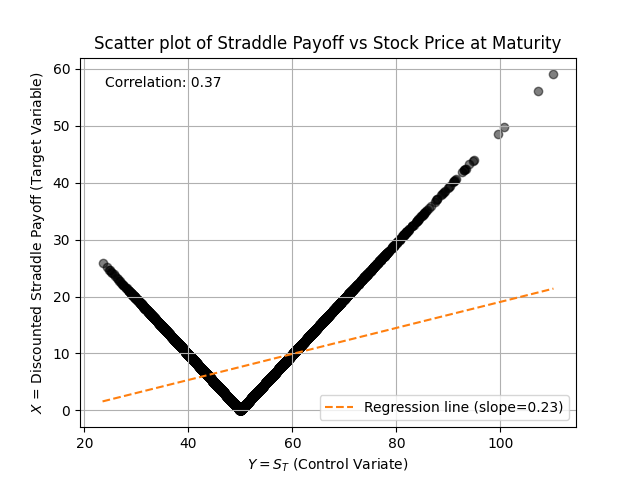
\includegraphics[width=0.6\textwidth]{assets/straddle-option-linear-scatter.png}
\caption{$h(S_T)$ vs $S_T$ for Straddle Option, $S_0 = K = 50$, using $Y = S_T$ as a control variate.}
\end{figure}
\begin{itemize}
    \item  Highly non-linear relationship between $X$ and $Y$ when $S_0 = K$.
    \item Reduced effectiveness of linear CV.
\end{itemize}
\end{frame}

% Straddle Option: quadratic control variate
\begin{frame}{Straddle Option: Control Variates (Quadratic)}
\small
Use two control variates: $Y_1 = S_T$, $Y_2 = S_T^2$. Then $\mathbb{E}[S_T^2] = E[S_T]^2 + \text{Var}(S_T) = S_0^2 e^{(2r + \sigma^2)T}$ so $E[Y_1]$ and $E[Y_2]$ are known.

\textbf{New Control Variate Estimator:} 
\[
\hat{v}_{\text{CV}} = \bar{X} - b_1^* (\bar{Y_1} - \mathbb{E}[Y_1]) - b_2^* (\bar{Y_2} - \mathbb{E}[Y_2]).
\]

\begin{figure}[ht]
\centering
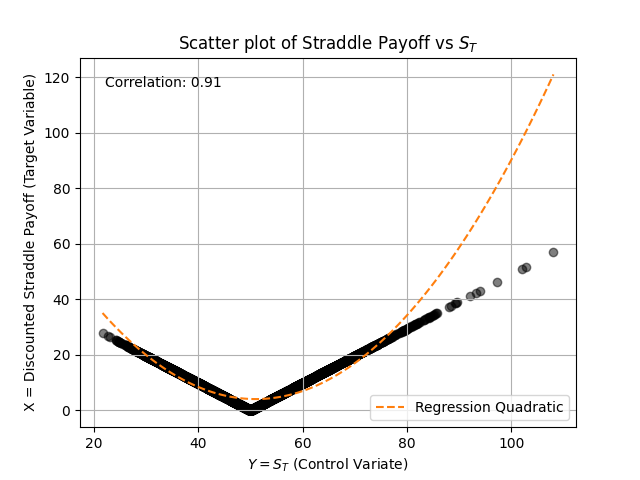
\includegraphics[width=0.6\textwidth]{assets/straddle-option-quadratic-scatter.png}
\caption{$h(S_T)$ vs $S_T$ with $S_0 = K = 50$, using $S_T$ and $S_T^2$ as control variates.}
\end{figure}

\end{frame}

\begin{frame}
\small
\textbf{Remark 1.} $b_1^*$ and $b_2^*$ computed via linear regression $X ~\sim Y_1 + Y_2$.

\textbf{Remark 2.} Adding quadratic term improves variance reduction significantly.
\begin{table}[h!]
\centering
\small
\begin{tabular}{l c c c}
\toprule
& Plain & CV & Better CV \\
\midrule
Estimate & 7.8795 & 7.8737 & $7.9489$ \\
S.E. & 0.0638 & 0.0593 & $0.0252$ \\
R.E. & 0.80\% & 0.75\% & $0.32\%$ \\
$\hat{\beta}^2$ & & 10.89\% & $83.93\%$ \\
\bottomrule
\end{tabular}
\caption{Straddle Option: comparison of linear and quadratic CV.}
\end{table}


\end{frame}


\begin{frame}{Control Variates: Limitations}
\small
\textbf{Generalization:}
\begin{itemize}
    \item Control Variate as linear combinations of features
    $$ Y' = \sum_{i = 1}^m b_i  \psi_i (Y)  $$
    $b_i$ chosen to minimize variance.
    \item Choice of functions $\psi_i$ in $\Phi(Y) = (\psi_1(Y),\dots,\psi_m(Y))$ affects efficiency of variance reduction.
    \item Require $\mathbb{E}[Y]$ to be known exactly.
    \item $\beta$ may be small $\rightarrow $ CV is less effective.
\end{itemize}

\metroset{block=fill}
\begin{alertblock}{Key Idea}
Replace linear combinations of basis functions with a \emph{rich function space} for variance reduction.
\end{alertblock}

\end{frame}

\subsection{Control Functionals}

\begin{frame}[fragile]{Control Functionals: Overview}
\small

\textit{Setup:} estimate $v = \mathbb{E}[h(Z)]$, where $Z \sim p(z)$.

\textbf{Control Variates:} approximates $h(z)$ by
\[
h(z) \approx g(z) = b_1 \psi_1(z) + \dots + b_m \psi_m(z),
\]

\begin{itemize}
\item $\mathbb{E}[\psi_i(Z)]$ are known.
\item Coefficients $b_i$ minimize the empirical error between $h(z)$ and $g(z)$ on $Z_i$.
\end{itemize}

\textbf{Control Functionals\cite{cf}:} approximates $h(z)$ by
$$h(z) \approx g(z) \in \mathcal{H}_+ \gg \text{span}(\psi_1, ..., \psi_m)$$

\begin{itemize}
    \item $\mathcal{H}_+$ is a \emph{Reproducing Kernel Hilbert Space} (RKHS) with a symm., p.d., kernel $k_+(\cdot, \cdot)$.
    \item Regularized Empirical Risk Functional:
    \[
    g^* = \arg \min_{g \in \mathcal{H}_+} \frac{1}{N} \sum_{i=1}^N \|h(Z_i) - g(Z_i)\|^2 + \lambda \|g\|_{\mathcal{H}_+}^2,
    \]
\end{itemize}

where $\lambda > 0$ is a regularization parameter controlling smoothness of $g$.

\end{frame}

\begin{frame}
\small

\metroset{block=fill}
\begin{alertblock}{Representer Theorem:} Any minimizer $g^*$ of the \textbf{\textit{regularized empirical risk functional}} admits a representation of the form
\[
g^*(z) = \sum_{i=1}^N b_i k_+(z, Z_i),
\]
for some coefficients $b_i \in \mathbb{R}$, \cite{ScholkopfSmola2002}.
\end{alertblock}

\textbf{CF Estimator:} 
\[
\hat{v}_{\rm CF} = \frac{1}{N} \sum_{i=1}^N \underbrace{h(Z_i) - g^*(Z_i)}_{\text{residuals}} + \mathbb{E}[g^*(Z)].
\]

\begin{itemize}
    \item Construct $k_+$ such that $\mathbb{E}[k_+(Z, Z_i)]$ is known or computed easily.
\end{itemize}
\end{frame}

\begin{frame}{Control Functionals: Stein Operators}
\small
\metroset{block=fill}
\begin{alertblock}{Stein Operator\cite{chen2011normal}}
    Given density $p$ and function $\phi$, the \textit{Stein Operator} $\mathcal{S}_p$ is defined as
    $$\mathcal{S}_p[\phi](z) = \nabla_z \cdot \phi(z) + \phi(z) \cdot \nabla_z \log p(z).$$
\end{alertblock}
\begin{itemize}
    \item \textbf{Zero-Mean Property} If $X$ has density $p$, then $\mathbb{E}[\mathcal{S}_p [\phi](X)] = 0$. 
    \item Apply $\mathcal{S}_p$ to both arguments of $k(\cdot, \cdot)$ to obtain a ``zero-mean kernel" $k_0(\cdot, \cdot)$.
\end{itemize}

\textbf{Modified RBF Kernel:} The standard normal density $p$ and a Radial Basis Function Kernel \textit{modified with a decay term}
$$k(z, z') = (1 + \alpha_1||z||^2 + \alpha_1 ||z'||^2)^{-1} \exp \left(-\frac{||z - z'||^2 }{2\alpha_2^2} \right),$$
where $\alpha_1, \alpha_2 > 0$ are the decay scale and length scale terms respectively. Then\footnote{See appendix for derivation.}
$$k_0(z, z') = k(z, z') \left(\frac{1 + ||z - z'||^2}{\alpha_2^2} + \frac{||z - z'||^2}{\alpha_2^4}  + \frac{2 \alpha_1(||z - z'||^2 + 2zz')}{1\ + \alpha_1 ||z||^2 + \alpha_1 ||z'||^2 }   + zz'  \right).$$

\end{frame}

\begin{frame}
\small
\begin{figure}
    \centering
    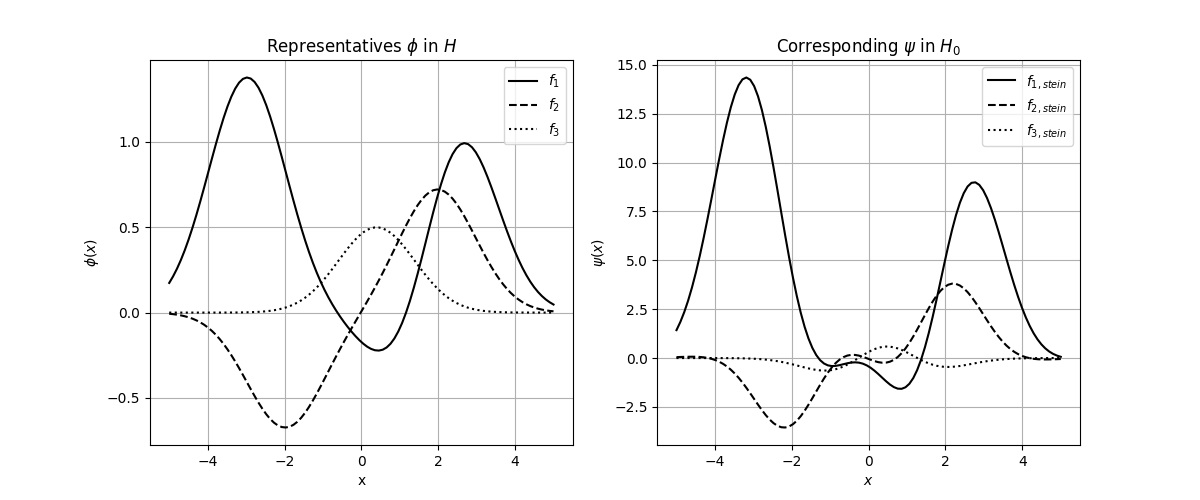
\includegraphics[width=1.0\linewidth]{assets/RKHS-kernel-functions.png}
    \caption{Elements of $\mathcal{H}$ and $\mathcal{H}_0$ for the standard normal distribution and modified RBF kernel with decay scale $\alpha_1 = 0.001$ and length scale $\alpha_2= 1.0$}
    \label{fig:rkhs-kernel-functions}
\end{figure}
\end{frame}

\begin{frame}{Control Functionals: Methodology}
\small

\textbf{Step 1: (Sample Splitting)} Draw $N$ i.i.d. samples $\{Z_i\}_{i=1}^N$ from $p(z)$ and split into:
\begin{itemize}
    \item \emph{Training set:} $\mathcal{D}_0 = \{Z_i\}_{i=1}^M$ $\rightarrow$ ``pilot sample"
    \item \emph{Test set:} $\mathcal{D}_1 = \{Z_i\}_{i=M+1}^N$
\end{itemize}

\vspace{0.5cm}

\textbf{Step 2: (Learn Control Functional)}  
Solve the regularized least squares (RLS) problem for $g^* \in \mathcal{H}_+$ on $\mathcal{D}_0$:
\begin{equation}
g^* = \arg \min_{g \in \mathcal{H}_+} \frac{1}{M} \sum_{i=1}^M \|h(Z_i) - g(Z_i)\|^2 + \lambda \|g\|_{\mathcal{H}_+}^2 \label{rls-eq} \tag{1} 
\end{equation}

\textbf{Parameters:} Choose $M$ such that $M/N \to \eta \in (0,1)$ and $\lambda = O(M^{-1/2})$.  


\end{frame}

\begin{frame}
\small
\textbf{Step 3: (Construct Estimator)}  
The control functional estimator on $\mathcal{D}_1$ is computed as:
\[
\hat{v}_{\rm CF} = \frac{1}{N-M} \mathbf{1}^T (\mathbf{h}_1 - \hat{\mathbf{h}}_1) + 
\underbrace{\frac{\mathbf{1}^T (\mathbf{K}_0 + \lambda M \mathbf{I})^{-1} \mathbf{h}_0}{1 + \mathbf{1}^T (\mathbf{K}_0 + \lambda M \mathbf{I})^{-1} \mathbf{1}}}_{\mathbb{E}[g^*(Z)]}
\]

where $$\mathbf{h}_0 = [h(Z_1), \dots, h(Z_M)]^T, \quad
\mathbf{h}_1 = [h(Z_{M+1}), \dots, h(Z_N)]^T,$$
$$\mathbf{1} = [1, \dots, 1]^T,
\quad
(\mathbf{K}_0)_{i,j} = k_0(Z_i, Z_j).
$$

The predictions on $\mathcal{D}_1$ are
$$\hat{\mathbf{h}}_1 = \mathbf{K}_{1,0} (\mathbf{K}_0 + \lambda M \mathbf{I})^{-1} \mathbf{h}_0 + (\mathbf{1} - \mathbf{K}_{1,0} (\mathbf{K}_0 + \lambda M \mathbf{I})^{-1} \mathbf{1}) 
\frac{\mathbf{1}^T (\mathbf{K}_0 + \lambda M \mathbf{I})^{-1} \mathbf{h}_0}{1 + \mathbf{1}^T (\mathbf{K}_0 + \lambda M \mathbf{I})^{-1} \mathbf{1}},
$$

with $(\mathbf{K}_{1,0})_{i,j} = k_0(Z_{M+i}, Z_j)$.
\vspace{0.3cm}

\metroset{block=fill}
\begin{alertblock}{Super-root-$N$ convergence.}
    Under regularity conditions on the kernel $k_0(\cdot, \cdot)$ and the density $p$, $\hat{v}_{\rm CF}$ achieves \emph{super-root-$N$ convergence}\cite{cf}. 
\end{alertblock}

\end{frame}

\begin{frame}{Straddle Option: Control Functionals}
\small
\textbf{Straddle Option:} Revisit the straddle option with $N=10{,}000$.

\textbf{CF Estimator:} \textit{modified RBF kernel} with parameters ($\alpha_1=0.001, \alpha_2=1, \eta=0.25$).  

\begin{figure}[h!]
\centering
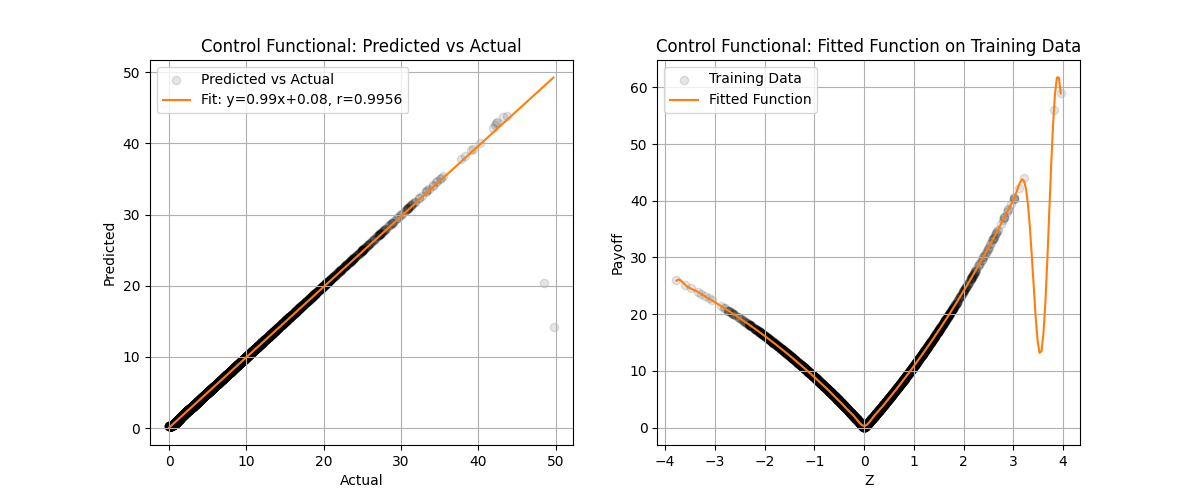
\includegraphics[width=1.0\textwidth]{assets/straddle-option-control-functionals-example.png}
\caption{Straddle Option Pricing: Control Functionals. High correlation between $\mathbf{h}_1$ and $\hat{\mathbf{h}}_1$ (left). Learned $g^*$ fits $h$ well (right).}
\end{figure}
\end{frame}

\begin{frame}
\small

\textbf{Remark 3.} CF Estimator outperforms the quadratic CV estimator.

\begin{table}[h!]
\centering
\small
\begin{tabular}{l c c c c c}
\toprule
& Plain & CV & Better CV & CF & Theoretical \\ 
\midrule
Estimate & 7.8795 & 7.8737 & 7.9489 & 7.9251 & 7.9260 \\
S.E. & 0.0638 & 0.0593 & 0.0252 & 0.0055 & - \\
R.E. & 0.80\% & 0.75\% & 0.32\% & 0.07\% & - \\
$\hat{\beta}^2$ & - & 10.89\% & 83.93\% & - & - \\
\bottomrule
\end{tabular}
\caption{Straddle Option: comparison of linear and quadratic CV with CF estimator.}
\end{table}

\end{frame}

\begin{frame}{Butterfly Multistrike Option: Control Functionals}
\small
\textbf{Butterfly Multistrike Option:} Deep out-of-the-money option. Discounted payoff:
$$ h(S_T) = e^{-rT} [ (S_T - K_1)^+ - 2 (S_T - K_2) + (S_T - K_3)^+].$$

\textbf{Parameters:} Strike prices: $K_1=90, K_2=100, K_3=120$
$$S_0=50, r=0.05, \sigma=0.3, T=1, \text{ and } N = 10{,}000.$$

\textbf{CF estimator:} \textit{modified RBF kernel} with parameters ($\alpha_1 = 0.001, \alpha_2 = 0.25, \eta = 0.4$)

\begin{figure}[h!]
\centering
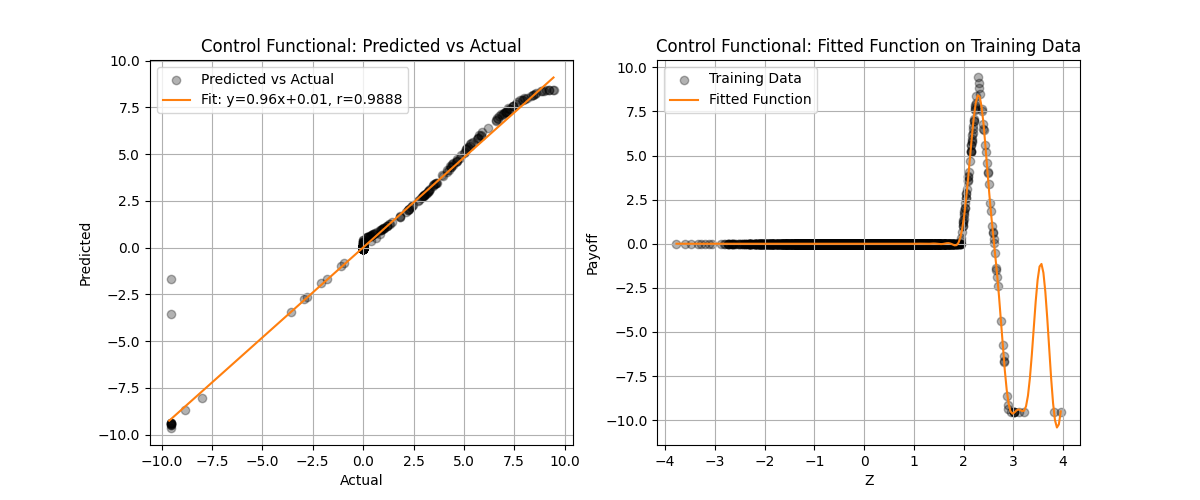
\includegraphics[width=1.0\textwidth]{assets/butterfly-strike-control-functionals-example.png}
\caption{Butterfly Multistrike Option Pricing: Control Functionals. High correlation between $\mathbf{h}_1$ and $\hat{\mathbf{h}}_1$ (left). Learned $g^*$ fits $h$ well (right).}
\end{figure}

\end{frame}

\begin{frame}
\small
\textbf{CV Estimator:} Same as before. $Y = S_T$
   
\begin{table}[h!]
\centering
\small
\begin{tabular}{l c c c c }
\toprule
& Plain & CV & CF & Theoretical \\ 
\midrule
Estimate & 0.0697 & 0.0687 & 0.0685 & 0.0683  \\
S.E. & 0.0087 & 0.0089 & 0.0020 & -  \\
R.E. & 12.46\% & 12.80\% & 2.93 \% & -  \\
\bottomrule
\end{tabular}
\caption{Butterfly Multistrike Option: Control Functional vs Plain Monte Carlo results}
\end{table}
\end{frame}


\begin{frame}{Control Functionals: Rate of Convergence}
\small
\textbf{CF estimator:} \textit{modified RBF Kernel} with parameters: ($\alpha_1 = 0.001, \alpha_2 = 0.25, \eta = 0.1$)
\begin{figure}
    \centering
    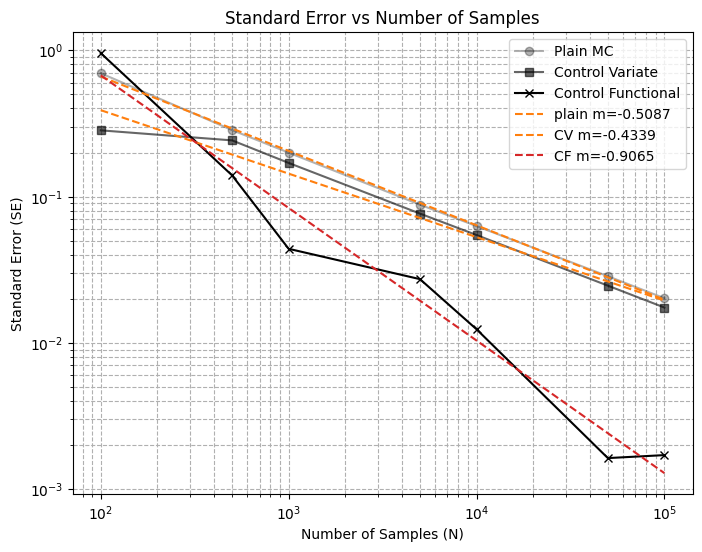
\includegraphics[width=0.75\linewidth]{assets/control-functional-se-vs-sample-size.png}
    \caption{Straddle Option: S.E. versus Sample Size $N$.}
\end{figure}

\end{frame}

\begin{frame}{Control Functionals: Limitations}
\small
\textbf{Computational Cost.} 
Solving the RLS problem in \eqref{rls-eq} requires inverting an $M \times M$ kernel matrix $K$, with computational cost $\mathcal{O}(M^3) \sim O(N^3)$ and memory cost $\mathcal{O}(M^2)$.
For large $M$, the variance reduction must be weighed against this cost.
\begin{itemize}
    \item Case: generating samples $h(X_i)$ expensive.
    \item Case: generating samples $h(X_i)$ cheap.
\end{itemize}

\textbf{Kernel Selection.} 
Performance is sensitive to the choice of $k_0$ and the regularization parameter $\lambda$.

\end{frame}

\begin{frame}
\small
\textbf{Theoretical Assumptions.} 
Super-root-$N$ convergence is guaranteed under certain conditions on the kernel $k_0$, the density $p$, and the dataset. 
\begin{itemize}
    \item Kernel $k_0(\cdot, \cdot)$ is bounded: $$\sup_{z \in \Omega} k_0(z, z) < \infty.$$
    Does not hold for standard RBF kernel:
    \[
        k(z, z') = \exp\Big(-\frac{\|z - z'\|^2}{2\alpha^2}\Big).
    \]
    \item Density is ``nice"; $p \in C^1(\Omega, \mathbb{R})$, not true for many \textit{useful} $p$, e.g. uniform dist.
\end{itemize}
\end{frame}



% \subsection{Importance Sampling}
% \begin{frame}{Importance Sampling: Overview}
% \small
% Importance sampling (IS) reduces variance by sampling more frequently from regions that contribute most to the expectation.

% \[
% \hat{v} = \frac{1}{N} \sum_{i=1}^N h(X_i), \quad X_i \sim f(x)
% \]

% \textbf{IS Estimator:}
% \[
% \hat{v}_{\text{IS}} = \frac{1}{N} \sum_{i=1}^N h(X_i) \frac{f(X_i)}{g(X_i)}, \quad X_i \sim g(x)
% \]

% \begin{itemize}
%     \item $f(X_i)/g(X_i)$ is the \emph{likelihood ratio} or \emph{importance weight}.
%     \item Commonly used in finance for rare-event probabilities (VaR, Expected Shortfall).
% \end{itemize}
% \end{frame}

% \begin{frame}{Variance Reduction in Importance Sampling}
% \small
% \begin{itemize}
%     \item Variance is minimized when samples are drawn from regions where $h(x) f(x)$ is large.
%     \item \textbf{Optimal (zero-variance) distribution:}
%     \[
%     g^*(x) = c |h(x)| f(x), \quad c = \frac{1}{\int |h(x)| f(x) dx} 
%     \]
%     \item Under $g^*$, $\text{Var}[\hat{v}_{\text{IS}}] = 0$.
%     \item Practical IS: restrict $g$ to a parametric family $ \mathcal{G} = \{ g(x; \theta) : \theta \in \mathbb{R}^d \} $.
%     \item Goal: find $\theta^*$ that minimizes KL divergence from $g^*$:
%     \[
%     \max_{g \in \mathcal{G}} \int h(x) f(x) \log g(x; \theta) dx.
%     \]
% \end{itemize}
% \end{frame}

% \begin{frame}{Mode Matching Heuristic}
% \small
% \begin{itemize}
%     \item Align the mode of $g(x; \theta)$ with the mode of $|h(x)| f(x)$.
%     \item Example: $g \sim \mathcal{N}(\mu, 1)$, set
%     \[
%     \mu^* = \arg \max_x |h(x)| f(x)
%     \]
%     \item Effective for unimodal target distributions.
% \end{itemize}

% \begin{figure}
% \centering
% 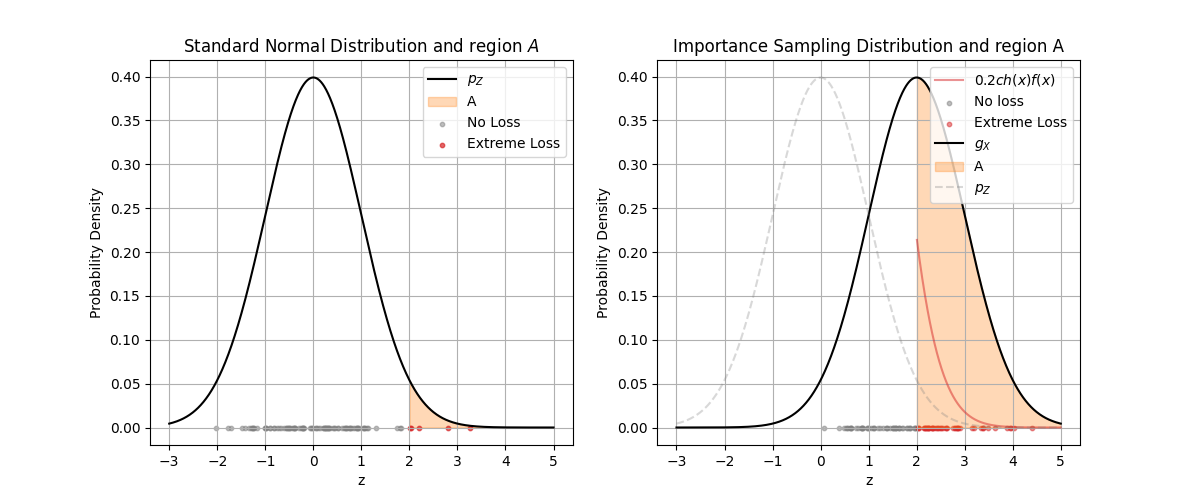
\includegraphics[width=1.0\textwidth]{assets/importance-sampling-illustration.png}
% \caption{Mode matching: shifting $g$ towards high-contribution region improves IS efficiency.}
% \end{figure}
% \end{frame}

% \begin{frame}{Iterative Cross-Entropy Method}
% \small
% \begin{itemize}
%     \item Gradient of KL objective w.r.t. $\theta$:
%     \[
%     \frac{\partial}{\partial \theta} L(\theta) = \int h(x) f(x) \frac{\partial}{\partial \theta} \log g(x; \theta) dx
%     \]
%     \item Approximated via Monte Carlo:
%     \[
%     \frac{1}{N} \sum_{i=1}^N h(X_i) \frac{f(X_i)}{g(X_i; \theta)} \frac{\partial}{\partial \theta} \log g(X_i; \theta)
%     \]
%     \item Iterative update: $\hat{\theta}_k \to \hat{\theta}_{k+1}$ until convergence.
%     \item Example (Normal family $g \sim \mathcal{N}(\mu, I_m)$):
%     \[
%     \hat{\mu}_{k+1} = \frac{\sum_i h(X_i) \ell_{\hat{\mu}_k}(X_i) X_i}{\sum_i h(X_i) \ell_{\hat{\mu}_k}(X_i)}, \quad \ell_{\hat{\mu}_k}(X_i) = \frac{f(X_i)}{g(X_i; \hat{\mu}_k)}
%     \]
% \end{itemize}
% \end{frame}

% \begin{frame}{Importance Sampling: Deep Out-of-the-Money Options}
% \small
% Deep out-of-the-money options are challenging to price accurately with standard Monte Carlo due to low exercise probability.

% \begin{itemize}
%     \item IS focuses sampling on the tail regions of the underlying distribution.
%     \item Consider a European call option:
%     \[
%     S_0 = 50, \quad r = 0.05, \quad \sigma = 0.2, \quad T = 1
%     \]
%     \item Compare Plain MC vs IS across strike prices $K = 80, 100, 120$.
% \end{itemize}
% \end{frame}

% \begin{frame}{Choosing the Importance Sampling Distribution}
% \small
% \begin{itemize}
%     \item Alternative distribution $g$ chosen via \textbf{mode matching} from $ \mathcal{G} = \{ N(\mu, 1) : \mu \in \mathbb{R} \} $.
%     \item Solve for $\mu^*$ numerically:
%     \[
%     S_0 e^{-1/2 \sigma^2 + \sigma \sqrt{T} \mu^*} (\sigma \sqrt{T} - \mu^*) + e^{-r T} K \mu^* = 0
%     \]
%     \item Bisection method yields $\mu^* \approx 4.47$ for deep OTM options.
% \end{itemize}
% \end{frame}

% \begin{frame}{European Call Option: Pricing Results}
% \small
% \begin{table}[]
% \centering
% \begin{tabular}{c|cc|cc|cc}
% \hline
% Strike & Plain MC & IS & Plain MC & IS & Plain MC & IS \\ 
% $K$ & \multicolumn{2}{c|}{80} & \multicolumn{2}{c|}{100} & \multicolumn{2}{c}{120} \\ \hline
% Theoretical & 0.079477 & - & 0.002399 & - & 0.000061 & - \\
% Estimate & 0.073593 & 0.080079 & 0.005058 & 0.002373 & 0.000000 & 0.000060 \\
% S.E. & 0.008955 & 0.000808 & 0.002402 & 0.000030 & 0.000000 & 0.000001 \\
% R.E. & 12.17\% & 1.01\% & 47.48\% & 1.26\% & NaN & 1.45\% \\
% $\hat{\mu}$ & - & 2.6001 & - & 3.6014 & - & 4.4569 \\ \hline
% \end{tabular}
% \caption{European Call Option: Plain MC vs Importance Sampling.}
% \end{table}
% \end{frame}

% \begin{frame}{Importance Sampling: Payoff Distribution}
% \small
% \begin{figure}
% \centering
% 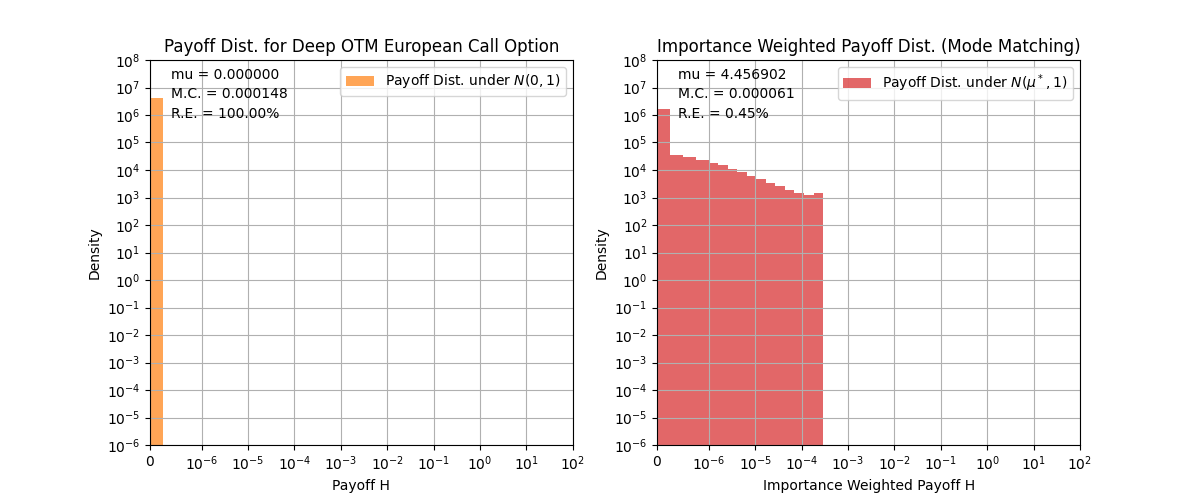
\includegraphics[width=1.0\textwidth]{assets/importance-sampling-european-call-option.png}
% \caption{Payoff distribution under the original and importance sampling distributions. IS concentrates samples in the tail, increasing non-zero payoffs.}
% \end{figure}

% \begin{itemize}
%     \item Sampling from $N(\mu^*, 1)$ concentrates samples in the critical region.
%     \item Leads to higher frequency of non-zero payoffs and reduced variance.
%     \item Importance sampling significantly outperforms plain MC in deep OTM scenarios.
% \end{itemize}
% \end{frame}


\section{Conclusion}

\begin{frame}[fragile]{Report}
\small
Get the full report and code from 

\begin{center}\url{github.com/chinzhening/capstone-project}\end{center}

An implementation of the Control Functionals Method for Modified RBF Kernel can be found at
\begin{center}\texttt{./src/control\_functionals\_implementation.py}
\end{center}

\begin{lstlisting}
class ControlFunctional:
    """A Control Functional model for variance reduction in Monte Carlo integration."""
    def __init__(self, X, Y, key, kernel_fn=modified_stein_rbf_kernel, eta=0.10, length_scale=1.0, decay_scale=1e-3):
        ...

    def fit(self, alpha=1e-3): ...
    def predict(self): ...
    def summary(self): ...
\end{lstlisting}
\end{frame}

{\setbeamercolor{palette primary}{fg=black, bg=white}
\begin{frame}[standout]
    Questions?
\end{frame}
}

\appendix

\begin{frame}[fragile]{Reproducing Kernel Hilbert Space}
\small
\textbf{Definition.} A Reproducing Kernel Hilbert Space (RKHS) is a Hilbert space of functions $\mathcal{H}$
in which evaluation at any point is a continuous linear functional.

\textbf{Reproducing Property.} There exists a positive definite kernel function $k(\cdot, \cdot)$ such that for all $f \in \mathcal{H}$ and $z \in \Omega$, we have
$$f(z) = \langle f, k(\cdot, z) \rangle_\mathcal{H}.$$
\end{frame}

\begin{frame}[fragile]{Construction of $k_+(\cdot, \cdot)$ via Stein Operators}
\small
\textbf{Step 1.} $k(\cdot, \cdot)$ to $k_0(\cdot, \cdot)$:
\begin{align*}
    k_0(z, z') &= \mathcal{S}_p^z \mathcal{S}_p^{z'}[k(z, z')] \\
\end{align*}
This can be expressed explicitly as
\begin{align*}
    k_0(z, z') &= \nabla_z \cdot \nabla_{z'} k(z, z')
    + u(z) \cdot \nabla_{z'} k(z, z') 
    + u(z') \cdot \nabla_z k(z, z') 
    + u(z) \cdot u(z') k(z, z').
\end{align*}
where $u(x) = \nabla_z \cdot \log p(z)$ is the score function of $p$.
\textbf{Note.} Kernel $k_0$ is p.d. \cite{cf} and satisfies zero-mean property:
\[
\int_\Omega k_0(z, z') \cdot p(z')\, dz' = 0.
\]
\textbf{Step 2.} $k_0(\cdot, \cdot)$ to $k_+(\cdot, \cdot)$:

Add space of constant functions $\mathcal{C} = \{c : c \in \mathbb{R}\}$ with associated kernel $k_C(z,z') = 1$
\[\mathcal{H}_+ = \mathcal{H}_0 + \mathcal{H}_C\]
\[
 k_+(z,z') = 1 + k_0(z,z').
\]
Then $\mathcal{H}_+$ is also a RKHS. Solving the RLS problem in (1) is equivalent to \hl{Regularized Kernel Regression} with $k_+(\cdot, \cdot)$.
\end{frame}

\begin{frame}[fragile]{Modified RBF Kernel $k(\cdot, \cdot) \rightarrow k_0(\cdot, \cdot)$}
\small
\textbf{Base modified RBF kernel:} 
\[
k(z, z') = \frac{\exp(-\|z - z'\|^2 / 2 \alpha_2^2)}{1 + \alpha_1 (\|z\|^2 + \|z'\|^2)}, 
\quad \alpha_1, \alpha_2 > 0
\]
\textbf{Standard Normal Density}
$$p(z) = (2\pi)^{-1} \exp(-z^2/2)$$

\vspace{0.5cm}
\textbf{Step 1.} Score function for standard normal: 
\[
u(z) = \nabla_z \log p(z) = -z \Rightarrow \mathcal{S}_p^z[\phi(z)] = \nabla_z \cdot \phi(z) - z \cdot \phi(z)
\]
    
\textbf{Step 2.} Apply Stein Operator to left argument $z$.
\[k_0(z, z') = \mathcal{S}_p^{z'} \mathcal{S}_p^{z} [k(z, z')]\]
\begin{align*}
\phi(z) = k(z, \cdot) \Rightarrow \nabla_z \cdot \phi(z) &= -\frac{\exp(-||z - z'||^2 / 2 \alpha_2^2)}{1 + \alpha_1 ||z ||^2 + \alpha_2 ||z\|^2}\left(\frac{z - z'}{\alpha_2^2} - \frac{2\alpha_1 z}{1 + \alpha_1 ||z||^2 + \alpha_1 ||z'||^2} \right) \\
&= -k(z, z') \left(\frac{z - z'}{\alpha_2^2} - \frac{2\alpha_1 z}{1 + \alpha_1 ||z||^2 + \alpha_1 ||z'||^2} \right)
\end{align*}
\end{frame}

\begin{frame}[fragile]
\small
Applying on the left.
\begin{align*}
\mathcal{S}_p^{z} [k(z, z')] &= -k(z, z')\left(\frac{z - z'}{\alpha_2^2} - \frac{2\alpha_1 z}{1 + \alpha_1 ||z||^2 + \alpha_1 ||z'||^2}{} \right)  - z \cdot k(z, z') \\
&= -k(z, z') \left( \frac{z -z'}{\alpha_2^2} + \frac{2 \alpha_1 z}{ 1 + \alpha_1 ||z||^2 + \alpha_1 ||z'||^2}+ z \right)
\end{align*}
\textbf{Step 3.} Apply Stein Operator to right argument $z'$.
\begin{align*}
\nabla_{z'} \cdot \mathcal{S}_p^{z} [k(z, z')] &= -k(z, z') \left( -\frac{1}{\alpha_2^2 } - \frac{4 \alpha_1^2 z z'}{(1 + \alpha_1 ||z||^2+ \alpha_1 ||z'||^2)^2} \right) \\& + k(z, z')\left( \frac{z' - z}{\alpha_2^2}-\frac{2 \alpha_1 z'}{1 + \alpha_1 ||z||^2+ \alpha_1 ||z'||^2}\right) \\
&= k(z, z') \left(\frac{1 + z' - z}{\alpha_2^2} + \frac{4 \alpha_1 z z' - 2 \alpha_1 z' (1 + \alpha_1 ||z||^2+ \alpha_1 ||z'||^2)}{(1 + \alpha_1 ||z||^2+ \alpha_1 ||z'||^2)^2} \right)
\end{align*}
\end{frame}

\begin{frame}[fragile]
\small
Apply to right argument $z'$:
\begin{align*}
\mathcal{S}_p^{z'}\mathcal{S}_p^{z} [k(z, z')]&= \mathcal{S}_p^{z'}\left[-k(z, z') \left( \frac{z -z'}{\alpha_2^2} + \frac{2 \alpha_1 z}{ 1 + \alpha_1 ||z||^2 + \alpha_1 ||z'||^2}+ z \right)\right]  \\
&= \cdots \\
&= k(z, z') \left(\frac{1 + ||z - z'||^2}{\alpha_2^2} + \frac{||z - z'||^2}{\alpha_2^4} + \frac{2\alpha_1 (||z - z-'||^2 + 2 z z')}{1 + \alpha_1 ||z||^2+ \alpha_1 ||z'||^2} + zz' \right)
\end{align*}
\end{frame}

\begin{frame}[fragile]{Control Functional Cost}
\small

\begin{figure}
    \centering
    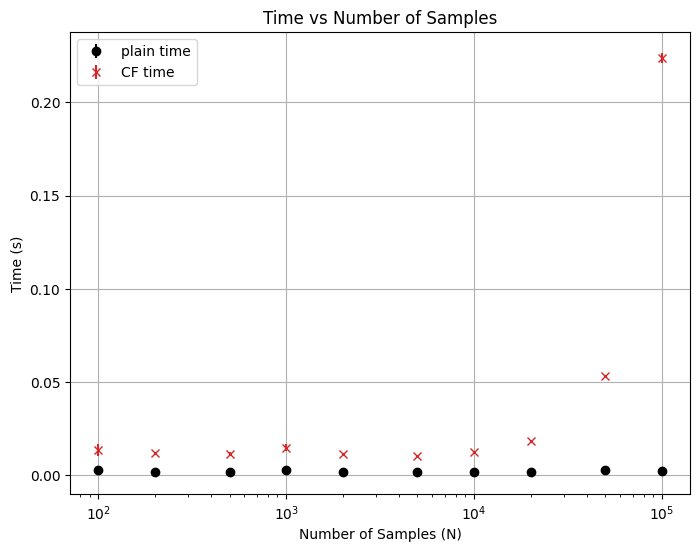
\includegraphics[width=0.75\linewidth]{assets/control-funtionals-computational-cost.png}
    \caption{Straddle Option: Computational Cost (time) versus Sample Size $N$}
\end{figure}

\end{frame}

\begin{frame}[allowframebreaks]{References}

  \bibliography{references}
  \bibliographystyle{abbrv}

\end{frame}

\end{document}
